\documentclass[border=5pt]{standalone}
\usepackage[T1]{fontenc}\usepackage{lmodern}\usepackage{pgfplots}
\pgfplotsset{compat=1.18}\begin{document}\sffamily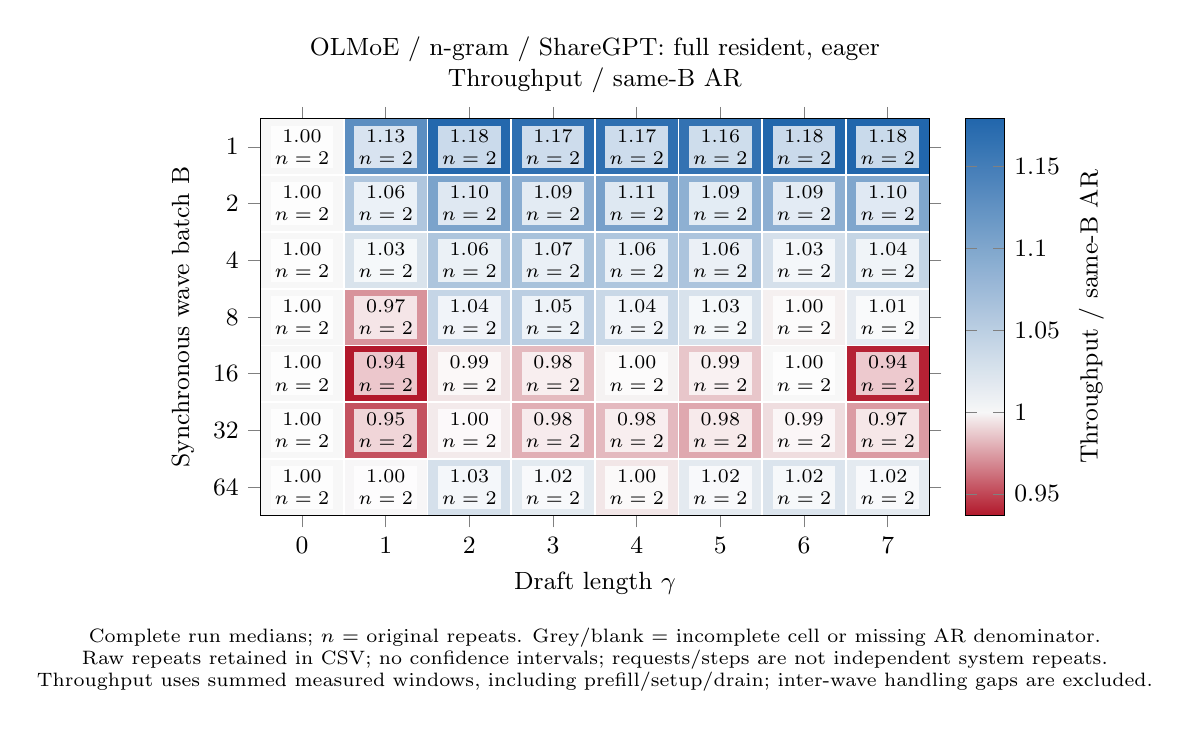
\begin{tikzpicture}
\begin{axis}[name=matrix,width=8.50cm,height=5.04cm,scale only axis,xmin=-.5,xmax=7.5,ymin=-.5,ymax=6.5,y dir=reverse,axis on top,tick align=outside,xtick={0,1,2,3,4,5,6,7},xticklabels={0,1,2,3,4,5,6,7},ytick={0,1,2,3,4,5,6},yticklabels={1,2,4,8,16,32,64},xlabel={Draft length $\gamma$},ylabel={Synchronous wave batch B},title={OLMoE / n-gram / ShareGPT: full resident, eager\\Throughput / same-B AR},title style={align=center,font=\small},tick label style={font=\small},label style={font=\small},point meta min=0.936882417663,point meta max=1.17911797191,colormap={matrixcolors}{rgb255=(178,24,43); rgb255=(181,33,51); rgb255=(183,41,59); rgb255=(186,50,66); rgb255=(189,58,74); rgb255=(191,67,82); rgb255=(194,75,90); rgb255=(197,84,98); rgb255=(199,92,106); rgb255=(202,101,113); rgb255=(204,110,121); rgb255=(207,118,129); rgb255=(210,127,137); rgb255=(212,135,145); rgb255=(215,144,153); rgb255=(218,152,160); rgb255=(220,161,168); rgb255=(223,169,176); rgb255=(226,178,184); rgb255=(228,187,192); rgb255=(231,195,200); rgb255=(234,204,207); rgb255=(236,212,215); rgb255=(239,221,223); rgb255=(242,229,231); rgb255=(244,238,239); rgb255=(247,247,247); rgb255=(244,245,246); rgb255=(241,243,245); rgb255=(238,241,244); rgb255=(236,239,243); rgb255=(233,237,242); rgb255=(230,235,241); rgb255=(227,233,240); rgb255=(224,231,239); rgb255=(221,229,238); rgb255=(218,228,237); rgb255=(215,226,236); rgb255=(212,224,235); rgb255=(210,222,234); rgb255=(207,220,233); rgb255=(204,218,232); rgb255=(201,216,231); rgb255=(198,214,230); rgb255=(195,212,229); rgb255=(192,210,228); rgb255=(189,208,227); rgb255=(186,206,226); rgb255=(183,204,225); rgb255=(181,202,224); rgb255=(178,200,223); rgb255=(175,198,222); rgb255=(172,196,221); rgb255=(169,194,220); rgb255=(166,192,219); rgb255=(163,190,218); rgb255=(160,188,217); rgb255=(157,186,216); rgb255=(155,184,215); rgb255=(152,182,214); rgb255=(149,180,213); rgb255=(146,178,212); rgb255=(143,177,211); rgb255=(140,175,210); rgb255=(137,173,209); rgb255=(134,171,207); rgb255=(131,169,206); rgb255=(129,167,205); rgb255=(126,165,204); rgb255=(123,163,203); rgb255=(120,161,202); rgb255=(117,159,201); rgb255=(114,157,200); rgb255=(111,155,199); rgb255=(108,153,198); rgb255=(105,151,197); rgb255=(102,149,196); rgb255=(100,147,195); rgb255=(97,145,194); rgb255=(94,143,193); rgb255=(91,141,192); rgb255=(88,139,191); rgb255=(85,137,190); rgb255=(82,135,189); rgb255=(79,133,188); rgb255=(76,131,187); rgb255=(74,129,186); rgb255=(71,127,185); rgb255=(68,126,184); rgb255=(65,124,183); rgb255=(62,122,182); rgb255=(59,120,181); rgb255=(56,118,180); rgb255=(53,116,179); rgb255=(50,114,178); rgb255=(47,112,177); rgb255=(45,110,176); rgb255=(42,108,175); rgb255=(39,106,174); rgb255=(36,104,173); rgb255=(33,102,172)},colorbar,colorbar style={ylabel={Throughput / same-B AR},label style={font=\small},tick label style={font=\small}}]
\path[fill={rgb,255:red,247;green,247;blue,247},draw=white,line width=.6pt] (axis cs:-0.5,-0.5) rectangle (axis cs:0.5,0.5);
\node[align=center,font=\scriptsize,fill=white,fill opacity=.76,text opacity=1,inner sep=1.5pt] at (axis cs:0,0) {1.00\\$n=2$};
\path[fill={rgb,255:red,92;green,142;blue,193},draw=white,line width=.6pt] (axis cs:0.5,-0.5) rectangle (axis cs:1.5,0.5);
\node[align=center,font=\scriptsize,fill=white,fill opacity=.76,text opacity=1,inner sep=1.5pt] at (axis cs:1,0) {1.13\\$n=2$};
\path[fill={rgb,255:red,36;green,104;blue,173},draw=white,line width=.6pt] (axis cs:1.5,-0.5) rectangle (axis cs:2.5,0.5);
\node[align=center,font=\scriptsize,fill=white,fill opacity=.76,text opacity=1,inner sep=1.5pt] at (axis cs:2,0) {1.18\\$n=2$};
\path[fill={rgb,255:red,46;green,111;blue,177},draw=white,line width=.6pt] (axis cs:2.5,-0.5) rectangle (axis cs:3.5,0.5);
\node[align=center,font=\scriptsize,fill=white,fill opacity=.76,text opacity=1,inner sep=1.5pt] at (axis cs:3,0) {1.17\\$n=2$};
\path[fill={rgb,255:red,46;green,111;blue,177},draw=white,line width=.6pt] (axis cs:3.5,-0.5) rectangle (axis cs:4.5,0.5);
\node[align=center,font=\scriptsize,fill=white,fill opacity=.76,text opacity=1,inner sep=1.5pt] at (axis cs:4,0) {1.17\\$n=2$};
\path[fill={rgb,255:red,51;green,114;blue,178},draw=white,line width=.6pt] (axis cs:4.5,-0.5) rectangle (axis cs:5.5,0.5);
\node[align=center,font=\scriptsize,fill=white,fill opacity=.76,text opacity=1,inner sep=1.5pt] at (axis cs:5,0) {1.16\\$n=2$};
\path[fill={rgb,255:red,34;green,103;blue,172},draw=white,line width=.6pt] (axis cs:5.5,-0.5) rectangle (axis cs:6.5,0.5);
\node[align=center,font=\scriptsize,fill=white,fill opacity=.76,text opacity=1,inner sep=1.5pt] at (axis cs:6,0) {1.18\\$n=2$};
\path[fill={rgb,255:red,33;green,102;blue,172},draw=white,line width=.6pt] (axis cs:6.5,-0.5) rectangle (axis cs:7.5,0.5);
\node[align=center,font=\scriptsize,fill=white,fill opacity=.76,text opacity=1,inner sep=1.5pt] at (axis cs:7,0) {1.18\\$n=2$};
\path[fill={rgb,255:red,247;green,247;blue,247},draw=white,line width=.6pt] (axis cs:-0.5,0.5) rectangle (axis cs:0.5,1.5);
\node[align=center,font=\scriptsize,fill=white,fill opacity=.76,text opacity=1,inner sep=1.5pt] at (axis cs:0,1) {1.00\\$n=2$};
\path[fill={rgb,255:red,175;green,198;blue,222},draw=white,line width=.6pt] (axis cs:0.5,0.5) rectangle (axis cs:1.5,1.5);
\node[align=center,font=\scriptsize,fill=white,fill opacity=.76,text opacity=1,inner sep=1.5pt] at (axis cs:1,1) {1.06\\$n=2$};
\path[fill={rgb,255:red,123;green,163;blue,203},draw=white,line width=.6pt] (axis cs:1.5,0.5) rectangle (axis cs:2.5,1.5);
\node[align=center,font=\scriptsize,fill=white,fill opacity=.76,text opacity=1,inner sep=1.5pt] at (axis cs:2,1) {1.10\\$n=2$};
\path[fill={rgb,255:red,138;green,173;blue,209},draw=white,line width=.6pt] (axis cs:2.5,0.5) rectangle (axis cs:3.5,1.5);
\node[align=center,font=\scriptsize,fill=white,fill opacity=.76,text opacity=1,inner sep=1.5pt] at (axis cs:3,1) {1.09\\$n=2$};
\path[fill={rgb,255:red,119;green,160;blue,202},draw=white,line width=.6pt] (axis cs:3.5,0.5) rectangle (axis cs:4.5,1.5);
\node[align=center,font=\scriptsize,fill=white,fill opacity=.76,text opacity=1,inner sep=1.5pt] at (axis cs:4,1) {1.11\\$n=2$};
\path[fill={rgb,255:red,142;green,176;blue,210},draw=white,line width=.6pt] (axis cs:4.5,0.5) rectangle (axis cs:5.5,1.5);
\node[align=center,font=\scriptsize,fill=white,fill opacity=.76,text opacity=1,inner sep=1.5pt] at (axis cs:5,1) {1.09\\$n=2$};
\path[fill={rgb,255:red,141;green,175;blue,210},draw=white,line width=.6pt] (axis cs:5.5,0.5) rectangle (axis cs:6.5,1.5);
\node[align=center,font=\scriptsize,fill=white,fill opacity=.76,text opacity=1,inner sep=1.5pt] at (axis cs:6,1) {1.09\\$n=2$};
\path[fill={rgb,255:red,127;green,166;blue,205},draw=white,line width=.6pt] (axis cs:6.5,0.5) rectangle (axis cs:7.5,1.5);
\node[align=center,font=\scriptsize,fill=white,fill opacity=.76,text opacity=1,inner sep=1.5pt] at (axis cs:7,1) {1.10\\$n=2$};
\path[fill={rgb,255:red,247;green,247;blue,247},draw=white,line width=.6pt] (axis cs:-0.5,1.5) rectangle (axis cs:0.5,2.5);
\node[align=center,font=\scriptsize,fill=white,fill opacity=.76,text opacity=1,inner sep=1.5pt] at (axis cs:0,2) {1.00\\$n=2$};
\path[fill={rgb,255:red,217;green,227;blue,236},draw=white,line width=.6pt] (axis cs:0.5,1.5) rectangle (axis cs:1.5,2.5);
\node[align=center,font=\scriptsize,fill=white,fill opacity=.76,text opacity=1,inner sep=1.5pt] at (axis cs:1,2) {1.03\\$n=2$};
\path[fill={rgb,255:red,173;green,197;blue,221},draw=white,line width=.6pt] (axis cs:1.5,1.5) rectangle (axis cs:2.5,2.5);
\node[align=center,font=\scriptsize,fill=white,fill opacity=.76,text opacity=1,inner sep=1.5pt] at (axis cs:2,2) {1.06\\$n=2$};
\path[fill={rgb,255:red,168;green,194;blue,219},draw=white,line width=.6pt] (axis cs:2.5,1.5) rectangle (axis cs:3.5,2.5);
\node[align=center,font=\scriptsize,fill=white,fill opacity=.76,text opacity=1,inner sep=1.5pt] at (axis cs:3,2) {1.07\\$n=2$};
\path[fill={rgb,255:red,174;green,198;blue,222},draw=white,line width=.6pt] (axis cs:3.5,1.5) rectangle (axis cs:4.5,2.5);
\node[align=center,font=\scriptsize,fill=white,fill opacity=.76,text opacity=1,inner sep=1.5pt] at (axis cs:4,2) {1.06\\$n=2$};
\path[fill={rgb,255:red,172;green,196;blue,221},draw=white,line width=.6pt] (axis cs:4.5,1.5) rectangle (axis cs:5.5,2.5);
\node[align=center,font=\scriptsize,fill=white,fill opacity=.76,text opacity=1,inner sep=1.5pt] at (axis cs:5,2) {1.06\\$n=2$};
\path[fill={rgb,255:red,213;green,224;blue,235},draw=white,line width=.6pt] (axis cs:5.5,1.5) rectangle (axis cs:6.5,2.5);
\node[align=center,font=\scriptsize,fill=white,fill opacity=.76,text opacity=1,inner sep=1.5pt] at (axis cs:6,2) {1.03\\$n=2$};
\path[fill={rgb,255:red,196;green,213;blue,229},draw=white,line width=.6pt] (axis cs:6.5,1.5) rectangle (axis cs:7.5,2.5);
\node[align=center,font=\scriptsize,fill=white,fill opacity=.76,text opacity=1,inner sep=1.5pt] at (axis cs:7,2) {1.04\\$n=2$};
\path[fill={rgb,255:red,247;green,247;blue,247},draw=white,line width=.6pt] (axis cs:-0.5,2.5) rectangle (axis cs:0.5,3.5);
\node[align=center,font=\scriptsize,fill=white,fill opacity=.76,text opacity=1,inner sep=1.5pt] at (axis cs:0,3) {1.00\\$n=2$};
\path[fill={rgb,255:red,216;green,147;blue,155},draw=white,line width=.6pt] (axis cs:0.5,2.5) rectangle (axis cs:1.5,3.5);
\node[align=center,font=\scriptsize,fill=white,fill opacity=.76,text opacity=1,inner sep=1.5pt] at (axis cs:1,3) {0.97\\$n=2$};
\path[fill={rgb,255:red,197;green,213;blue,230},draw=white,line width=.6pt] (axis cs:1.5,2.5) rectangle (axis cs:2.5,3.5);
\node[align=center,font=\scriptsize,fill=white,fill opacity=.76,text opacity=1,inner sep=1.5pt] at (axis cs:2,3) {1.04\\$n=2$};
\path[fill={rgb,255:red,187;green,206;blue,226},draw=white,line width=.6pt] (axis cs:2.5,2.5) rectangle (axis cs:3.5,3.5);
\node[align=center,font=\scriptsize,fill=white,fill opacity=.76,text opacity=1,inner sep=1.5pt] at (axis cs:3,3) {1.05\\$n=2$};
\path[fill={rgb,255:red,201;green,216;blue,231},draw=white,line width=.6pt] (axis cs:3.5,2.5) rectangle (axis cs:4.5,3.5);
\node[align=center,font=\scriptsize,fill=white,fill opacity=.76,text opacity=1,inner sep=1.5pt] at (axis cs:4,3) {1.04\\$n=2$};
\path[fill={rgb,255:red,216;green,226;blue,236},draw=white,line width=.6pt] (axis cs:4.5,2.5) rectangle (axis cs:5.5,3.5);
\node[align=center,font=\scriptsize,fill=white,fill opacity=.76,text opacity=1,inner sep=1.5pt] at (axis cs:5,3) {1.03\\$n=2$};
\path[fill={rgb,255:red,245;green,240;blue,240},draw=white,line width=.6pt] (axis cs:5.5,2.5) rectangle (axis cs:6.5,3.5);
\node[align=center,font=\scriptsize,fill=white,fill opacity=.76,text opacity=1,inner sep=1.5pt] at (axis cs:6,3) {1.00\\$n=2$};
\path[fill={rgb,255:red,230;green,235;blue,241},draw=white,line width=.6pt] (axis cs:6.5,2.5) rectangle (axis cs:7.5,3.5);
\node[align=center,font=\scriptsize,fill=white,fill opacity=.76,text opacity=1,inner sep=1.5pt] at (axis cs:7,3) {1.01\\$n=2$};
\path[fill={rgb,255:red,247;green,247;blue,247},draw=white,line width=.6pt] (axis cs:-0.5,3.5) rectangle (axis cs:0.5,4.5);
\node[align=center,font=\scriptsize,fill=white,fill opacity=.76,text opacity=1,inner sep=1.5pt] at (axis cs:0,4) {1.00\\$n=2$};
\path[fill={rgb,255:red,178;green,24;blue,43},draw=white,line width=.6pt] (axis cs:0.5,3.5) rectangle (axis cs:1.5,4.5);
\node[align=center,font=\scriptsize,fill=white,fill opacity=.76,text opacity=1,inner sep=1.5pt] at (axis cs:1,4) {0.94\\$n=2$};
\path[fill={rgb,255:red,241;green,228;blue,229},draw=white,line width=.6pt] (axis cs:1.5,3.5) rectangle (axis cs:2.5,4.5);
\node[align=center,font=\scriptsize,fill=white,fill opacity=.76,text opacity=1,inner sep=1.5pt] at (axis cs:2,4) {0.99\\$n=2$};
\path[fill={rgb,255:red,228;green,186;blue,191},draw=white,line width=.6pt] (axis cs:2.5,3.5) rectangle (axis cs:3.5,4.5);
\node[align=center,font=\scriptsize,fill=white,fill opacity=.76,text opacity=1,inner sep=1.5pt] at (axis cs:3,4) {0.98\\$n=2$};
\path[fill={rgb,255:red,245;green,242;blue,242},draw=white,line width=.6pt] (axis cs:3.5,3.5) rectangle (axis cs:4.5,4.5);
\node[align=center,font=\scriptsize,fill=white,fill opacity=.76,text opacity=1,inner sep=1.5pt] at (axis cs:4,4) {1.00\\$n=2$};
\path[fill={rgb,255:red,232;green,198;blue,202},draw=white,line width=.6pt] (axis cs:4.5,3.5) rectangle (axis cs:5.5,4.5);
\node[align=center,font=\scriptsize,fill=white,fill opacity=.76,text opacity=1,inner sep=1.5pt] at (axis cs:5,4) {0.99\\$n=2$};
\path[fill={rgb,255:red,247;green,247;blue,247},draw=white,line width=.6pt] (axis cs:5.5,3.5) rectangle (axis cs:6.5,4.5);
\node[align=center,font=\scriptsize,fill=white,fill opacity=.76,text opacity=1,inner sep=1.5pt] at (axis cs:6,4) {1.00\\$n=2$};
\path[fill={rgb,255:red,181;green,33;blue,52},draw=white,line width=.6pt] (axis cs:6.5,3.5) rectangle (axis cs:7.5,4.5);
\node[align=center,font=\scriptsize,fill=white,fill opacity=.76,text opacity=1,inner sep=1.5pt] at (axis cs:7,4) {0.94\\$n=2$};
\path[fill={rgb,255:red,247;green,247;blue,247},draw=white,line width=.6pt] (axis cs:-0.5,4.5) rectangle (axis cs:0.5,5.5);
\node[align=center,font=\scriptsize,fill=white,fill opacity=.76,text opacity=1,inner sep=1.5pt] at (axis cs:0,5) {1.00\\$n=2$};
\path[fill={rgb,255:red,196;green,81;blue,95},draw=white,line width=.6pt] (axis cs:0.5,4.5) rectangle (axis cs:1.5,5.5);
\node[align=center,font=\scriptsize,fill=white,fill opacity=.76,text opacity=1,inner sep=1.5pt] at (axis cs:1,5) {0.95\\$n=2$};
\path[fill={rgb,255:red,243;green,234;blue,235},draw=white,line width=.6pt] (axis cs:1.5,4.5) rectangle (axis cs:2.5,5.5);
\node[align=center,font=\scriptsize,fill=white,fill opacity=.76,text opacity=1,inner sep=1.5pt] at (axis cs:2,5) {1.00\\$n=2$};
\path[fill={rgb,255:red,225;green,175;blue,181},draw=white,line width=.6pt] (axis cs:2.5,4.5) rectangle (axis cs:3.5,5.5);
\node[align=center,font=\scriptsize,fill=white,fill opacity=.76,text opacity=1,inner sep=1.5pt] at (axis cs:3,5) {0.98\\$n=2$};
\path[fill={rgb,255:red,228;green,185;blue,191},draw=white,line width=.6pt] (axis cs:3.5,4.5) rectangle (axis cs:4.5,5.5);
\node[align=center,font=\scriptsize,fill=white,fill opacity=.76,text opacity=1,inner sep=1.5pt] at (axis cs:4,5) {0.98\\$n=2$};
\path[fill={rgb,255:red,223;green,168;blue,175},draw=white,line width=.6pt] (axis cs:4.5,4.5) rectangle (axis cs:5.5,5.5);
\node[align=center,font=\scriptsize,fill=white,fill opacity=.76,text opacity=1,inner sep=1.5pt] at (axis cs:5,5) {0.98\\$n=2$};
\path[fill={rgb,255:red,239;green,221;blue,223},draw=white,line width=.6pt] (axis cs:5.5,4.5) rectangle (axis cs:6.5,5.5);
\node[align=center,font=\scriptsize,fill=white,fill opacity=.76,text opacity=1,inner sep=1.5pt] at (axis cs:6,5) {0.99\\$n=2$};
\path[fill={rgb,255:red,219;green,155;blue,163},draw=white,line width=.6pt] (axis cs:6.5,4.5) rectangle (axis cs:7.5,5.5);
\node[align=center,font=\scriptsize,fill=white,fill opacity=.76,text opacity=1,inner sep=1.5pt] at (axis cs:7,5) {0.97\\$n=2$};
\path[fill={rgb,255:red,247;green,247;blue,247},draw=white,line width=.6pt] (axis cs:-0.5,5.5) rectangle (axis cs:0.5,6.5);
\node[align=center,font=\scriptsize,fill=white,fill opacity=.76,text opacity=1,inner sep=1.5pt] at (axis cs:0,6) {1.00\\$n=2$};
\path[fill={rgb,255:red,247;green,246;blue,247},draw=white,line width=.6pt] (axis cs:0.5,5.5) rectangle (axis cs:1.5,6.5);
\node[align=center,font=\scriptsize,fill=white,fill opacity=.76,text opacity=1,inner sep=1.5pt] at (axis cs:1,6) {1.00\\$n=2$};
\path[fill={rgb,255:red,213;green,224;blue,235},draw=white,line width=.6pt] (axis cs:1.5,5.5) rectangle (axis cs:2.5,6.5);
\node[align=center,font=\scriptsize,fill=white,fill opacity=.76,text opacity=1,inner sep=1.5pt] at (axis cs:2,6) {1.03\\$n=2$};
\path[fill={rgb,255:red,227;green,234;blue,240},draw=white,line width=.6pt] (axis cs:2.5,5.5) rectangle (axis cs:3.5,6.5);
\node[align=center,font=\scriptsize,fill=white,fill opacity=.76,text opacity=1,inner sep=1.5pt] at (axis cs:3,6) {1.02\\$n=2$};
\path[fill={rgb,255:red,242;green,230;blue,231},draw=white,line width=.6pt] (axis cs:3.5,5.5) rectangle (axis cs:4.5,6.5);
\node[align=center,font=\scriptsize,fill=white,fill opacity=.76,text opacity=1,inner sep=1.5pt] at (axis cs:4,6) {1.00\\$n=2$};
\path[fill={rgb,255:red,228;green,234;blue,240},draw=white,line width=.6pt] (axis cs:4.5,5.5) rectangle (axis cs:5.5,6.5);
\node[align=center,font=\scriptsize,fill=white,fill opacity=.76,text opacity=1,inner sep=1.5pt] at (axis cs:5,6) {1.02\\$n=2$};
\path[fill={rgb,255:red,219;green,228;blue,237},draw=white,line width=.6pt] (axis cs:5.5,5.5) rectangle (axis cs:6.5,6.5);
\node[align=center,font=\scriptsize,fill=white,fill opacity=.76,text opacity=1,inner sep=1.5pt] at (axis cs:6,6) {1.02\\$n=2$};
\path[fill={rgb,255:red,228;green,234;blue,240},draw=white,line width=.6pt] (axis cs:6.5,5.5) rectangle (axis cs:7.5,6.5);
\node[align=center,font=\scriptsize,fill=white,fill opacity=.76,text opacity=1,inner sep=1.5pt] at (axis cs:7,6) {1.02\\$n=2$};
\end{axis}
\node[below=1.3cm,align=center,font=\scriptsize] at (matrix.south) {Complete run medians; $n$ = original repeats. Grey/blank = incomplete cell or missing AR denominator.\\Raw repeats retained in CSV; no confidence intervals; requests/steps are not independent system repeats.\\Throughput uses summed measured windows, including prefill/setup/drain; inter-wave handling gaps are excluded.};
\end{tikzpicture}\end{document}
